% Options for packages loaded elsewhere
\PassOptionsToPackage{unicode}{hyperref}
\PassOptionsToPackage{hyphens}{url}
%
\documentclass[
]{article}
\usepackage{amsmath,amssymb}
\usepackage{iftex}
\ifPDFTeX
  \usepackage[T1]{fontenc}
  \usepackage[utf8]{inputenc}
  \usepackage{textcomp} % provide euro and other symbols
\else % if luatex or xetex
  \usepackage{unicode-math} % this also loads fontspec
  \defaultfontfeatures{Scale=MatchLowercase}
  \defaultfontfeatures[\rmfamily]{Ligatures=TeX,Scale=1}
\fi
\usepackage{lmodern}
\ifPDFTeX\else
  % xetex/luatex font selection
\fi
% Use upquote if available, for straight quotes in verbatim environments
\IfFileExists{upquote.sty}{\usepackage{upquote}}{}
\IfFileExists{microtype.sty}{% use microtype if available
  \usepackage[]{microtype}
  \UseMicrotypeSet[protrusion]{basicmath} % disable protrusion for tt fonts
}{}
\makeatletter
\@ifundefined{KOMAClassName}{% if non-KOMA class
  \IfFileExists{parskip.sty}{%
    \usepackage{parskip}
  }{% else
    \setlength{\parindent}{0pt}
    \setlength{\parskip}{6pt plus 2pt minus 1pt}}
}{% if KOMA class
  \KOMAoptions{parskip=half}}
\makeatother
\usepackage{xcolor}
\usepackage[margin=1in]{geometry}
\usepackage{color}
\usepackage{fancyvrb}
\newcommand{\VerbBar}{|}
\newcommand{\VERB}{\Verb[commandchars=\\\{\}]}
\DefineVerbatimEnvironment{Highlighting}{Verbatim}{commandchars=\\\{\}}
% Add ',fontsize=\small' for more characters per line
\usepackage{framed}
\definecolor{shadecolor}{RGB}{248,248,248}
\newenvironment{Shaded}{\begin{snugshade}}{\end{snugshade}}
\newcommand{\AlertTok}[1]{\textcolor[rgb]{0.94,0.16,0.16}{#1}}
\newcommand{\AnnotationTok}[1]{\textcolor[rgb]{0.56,0.35,0.01}{\textbf{\textit{#1}}}}
\newcommand{\AttributeTok}[1]{\textcolor[rgb]{0.13,0.29,0.53}{#1}}
\newcommand{\BaseNTok}[1]{\textcolor[rgb]{0.00,0.00,0.81}{#1}}
\newcommand{\BuiltInTok}[1]{#1}
\newcommand{\CharTok}[1]{\textcolor[rgb]{0.31,0.60,0.02}{#1}}
\newcommand{\CommentTok}[1]{\textcolor[rgb]{0.56,0.35,0.01}{\textit{#1}}}
\newcommand{\CommentVarTok}[1]{\textcolor[rgb]{0.56,0.35,0.01}{\textbf{\textit{#1}}}}
\newcommand{\ConstantTok}[1]{\textcolor[rgb]{0.56,0.35,0.01}{#1}}
\newcommand{\ControlFlowTok}[1]{\textcolor[rgb]{0.13,0.29,0.53}{\textbf{#1}}}
\newcommand{\DataTypeTok}[1]{\textcolor[rgb]{0.13,0.29,0.53}{#1}}
\newcommand{\DecValTok}[1]{\textcolor[rgb]{0.00,0.00,0.81}{#1}}
\newcommand{\DocumentationTok}[1]{\textcolor[rgb]{0.56,0.35,0.01}{\textbf{\textit{#1}}}}
\newcommand{\ErrorTok}[1]{\textcolor[rgb]{0.64,0.00,0.00}{\textbf{#1}}}
\newcommand{\ExtensionTok}[1]{#1}
\newcommand{\FloatTok}[1]{\textcolor[rgb]{0.00,0.00,0.81}{#1}}
\newcommand{\FunctionTok}[1]{\textcolor[rgb]{0.13,0.29,0.53}{\textbf{#1}}}
\newcommand{\ImportTok}[1]{#1}
\newcommand{\InformationTok}[1]{\textcolor[rgb]{0.56,0.35,0.01}{\textbf{\textit{#1}}}}
\newcommand{\KeywordTok}[1]{\textcolor[rgb]{0.13,0.29,0.53}{\textbf{#1}}}
\newcommand{\NormalTok}[1]{#1}
\newcommand{\OperatorTok}[1]{\textcolor[rgb]{0.81,0.36,0.00}{\textbf{#1}}}
\newcommand{\OtherTok}[1]{\textcolor[rgb]{0.56,0.35,0.01}{#1}}
\newcommand{\PreprocessorTok}[1]{\textcolor[rgb]{0.56,0.35,0.01}{\textit{#1}}}
\newcommand{\RegionMarkerTok}[1]{#1}
\newcommand{\SpecialCharTok}[1]{\textcolor[rgb]{0.81,0.36,0.00}{\textbf{#1}}}
\newcommand{\SpecialStringTok}[1]{\textcolor[rgb]{0.31,0.60,0.02}{#1}}
\newcommand{\StringTok}[1]{\textcolor[rgb]{0.31,0.60,0.02}{#1}}
\newcommand{\VariableTok}[1]{\textcolor[rgb]{0.00,0.00,0.00}{#1}}
\newcommand{\VerbatimStringTok}[1]{\textcolor[rgb]{0.31,0.60,0.02}{#1}}
\newcommand{\WarningTok}[1]{\textcolor[rgb]{0.56,0.35,0.01}{\textbf{\textit{#1}}}}
\usepackage{graphicx}
\makeatletter
\def\maxwidth{\ifdim\Gin@nat@width>\linewidth\linewidth\else\Gin@nat@width\fi}
\def\maxheight{\ifdim\Gin@nat@height>\textheight\textheight\else\Gin@nat@height\fi}
\makeatother
% Scale images if necessary, so that they will not overflow the page
% margins by default, and it is still possible to overwrite the defaults
% using explicit options in \includegraphics[width, height, ...]{}
\setkeys{Gin}{width=\maxwidth,height=\maxheight,keepaspectratio}
% Set default figure placement to htbp
\makeatletter
\def\fps@figure{htbp}
\makeatother
\setlength{\emergencystretch}{3em} % prevent overfull lines
\providecommand{\tightlist}{%
  \setlength{\itemsep}{0pt}\setlength{\parskip}{0pt}}
\setcounter{secnumdepth}{-\maxdimen} % remove section numbering
\ifLuaTeX
  \usepackage{selnolig}  % disable illegal ligatures
\fi
\IfFileExists{bookmark.sty}{\usepackage{bookmark}}{\usepackage{hyperref}}
\IfFileExists{xurl.sty}{\usepackage{xurl}}{} % add URL line breaks if available
\urlstyle{same}
\hypersetup{
  pdftitle={Norm\_Imputation\_strategy\_selection},
  pdfauthor={Fay},
  hidelinks,
  pdfcreator={LaTeX via pandoc}}

\title{Norm\_Imputation\_strategy\_selection}
\author{Fay}
\date{2023-09-28}

\begin{document}
\maketitle

\hypertarget{normalize-or-impute-first}{%
\section{Normalize or impute first?}\label{normalize-or-impute-first}}

Here is a document on selecting the best order for normalizationa and
imputation of the immune gene expression data.

\hypertarget{layout}{%
\subsection{Layout:}\label{layout}}

\begin{enumerate}
\def\labelenumi{\arabic{enumi}.}
\tightlist
\item
  Correlation of non-normalized and non-imputed gene expression data
\item
  Correlation of non-normalized and imputed gene expression data
\item
  Correlation of normalized data (no imputation)
\item
  Correlation of 1st normalized and sequentially imputed gene expression
  data
\item
  Corrrelation of 1st imputed and sequentially normalized gene
  expression data
\end{enumerate}

\hypertarget{data-input}{%
\subsection{Data input}\label{data-input}}

\hypertarget{libraries}{%
\subsubsection{Libraries}\label{libraries}}

\hypertarget{correlation-of-non-normalized-and-non-imputed-gene-expression-data}{%
\subsection{1. Correlation of non-normalized and non-imputed gene
expression
data}\label{correlation-of-non-normalized-and-non-imputed-gene-expression-data}}

\begin{Shaded}
\begin{Highlighting}[]
\NormalTok{gene\_correlation }\OtherTok{\textless{}{-}}\NormalTok{ lab }\SpecialCharTok{\%\textgreater{}\%} 
  \FunctionTok{filter}\NormalTok{(infection }\SpecialCharTok{==} \StringTok{"challenge"}\NormalTok{, dpi }\SpecialCharTok{==}\NormalTok{ max\_dpi) }\SpecialCharTok{\%\textgreater{}\%}
  \FunctionTok{ungroup}\NormalTok{() }\SpecialCharTok{\%\textgreater{}\%}
\NormalTok{  dplyr}\SpecialCharTok{::}\FunctionTok{select}\NormalTok{(}\FunctionTok{all\_of}\NormalTok{(Genes\_v))}

\CommentTok{\# draw correlation between the genes}
\NormalTok{gene\_correlation }\OtherTok{\textless{}{-}} \FunctionTok{as.matrix}\NormalTok{(}\FunctionTok{cor}\NormalTok{(gene\_correlation, }
                                  \AttributeTok{use=}\StringTok{"pairwise.complete.obs"}\NormalTok{))}

\CommentTok{\# load the function to calculate the p value for correlations}
\FunctionTok{source}\NormalTok{(}\StringTok{"R/Functions/p\_value\_for\_correlations.R"}\NormalTok{)}

\CommentTok{\# matrix of the p{-}value of the correlatio}
\NormalTok{p.mat }\OtherTok{\textless{}{-}} \FunctionTok{cor.mtest}\NormalTok{(gene\_correlation)}

\FunctionTok{corrplot}\NormalTok{(gene\_correlation, }
         \AttributeTok{method =} \StringTok{"circle"}\NormalTok{,  }\CommentTok{\#method of the plot, "color" would show colour gradient}
         \AttributeTok{tl.col =} \StringTok{"black"}\NormalTok{, }\AttributeTok{tl.srt=}\DecValTok{45}\NormalTok{, }\CommentTok{\#colour of labels and rotation}
         \AttributeTok{col =} \FunctionTok{brewer.pal}\NormalTok{(}\AttributeTok{n =} \DecValTok{8}\NormalTok{, }\AttributeTok{name =}\StringTok{"RdYlBu"}\NormalTok{), }\CommentTok{\#colour of matrix}
         \AttributeTok{order=}\StringTok{"hclust"}\NormalTok{, }\CommentTok{\#hclust reordering}
         \AttributeTok{p.mat =}\NormalTok{ p.mat, }\AttributeTok{sig.level =} \FloatTok{0.01}\NormalTok{, }\AttributeTok{insig =} \StringTok{"blank"}\NormalTok{,}
         \AttributeTok{addCoef.col =} \StringTok{\textquotesingle{}black\textquotesingle{}}\NormalTok{,}
         \AttributeTok{number.cex=}\FloatTok{0.5}\NormalTok{, }
         \AttributeTok{title =} \StringTok{"Lab"}\NormalTok{) }
\end{Highlighting}
\end{Shaded}

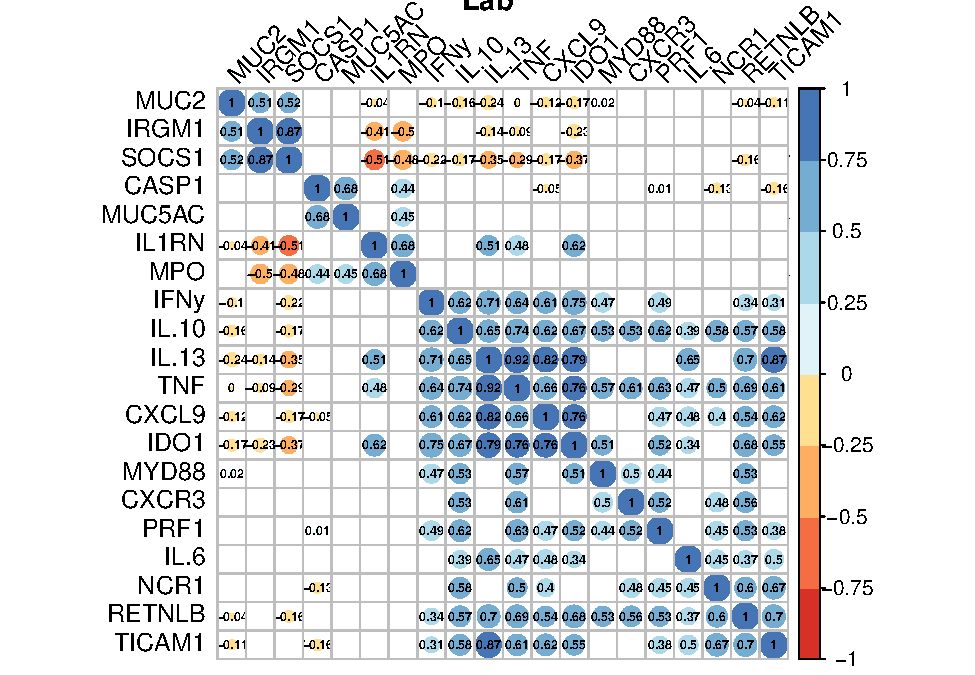
\includegraphics{Testing_normalization_imputation_order_files/figure-latex/unnamed-chunk-4-1.pdf}

\begin{Shaded}
\begin{Highlighting}[]
  \CommentTok{\#Add significance level to the correlogram}
\CommentTok{\#remove the values that are insignificant}
\end{Highlighting}
\end{Shaded}

\hypertarget{correlation-of-non-normalized-and-non-imputed-gene-expression-data-results}{%
\subsubsection{Correlation of non-normalized and non-imputed gene
expression data,
Results:}\label{correlation-of-non-normalized-and-non-imputed-gene-expression-data-results}}

\begin{enumerate}
\def\labelenumi{\alph{enumi}.}
\tightlist
\item
  positive correlations between MUC2, IRGM1 and SOCS1
\item
  positive correlations between CASP1 and MUC5AC
\item
  positive correlations between IFNy, IL.10, IL.13, TNF, CXCL9, TICAM1
  and IDO1
\item
  MYD88, PRF1, IL.6, NCR1, RETNLB, TICAM1 positve correlations with
  group c
\item
  negative correlations between group a (MUC2, IRGM1, SOCS1) and group c
  (IFNY, IL.10 etc)
\item
  negative correlations between IL1RN, MPO and group a
\item
  negative correlations between NCR1, RETNLB, TICAM1 and group a
\end{enumerate}

\hypertarget{correlation-of-non-normalized-and-imputed-gene-expression-data}{%
\subsection{2. Correlation of non-normalized and imputed gene expression
data}\label{correlation-of-non-normalized-and-imputed-gene-expression-data}}

\begin{Shaded}
\begin{Highlighting}[]
\NormalTok{lab }\OtherTok{\textless{}{-}}\NormalTok{ hm\_imp }\SpecialCharTok{\%\textgreater{}\%}
    \FunctionTok{filter}\NormalTok{(origin}\SpecialCharTok{==} \StringTok{"Lab"}\NormalTok{)}
\NormalTok{gene\_correlation }\OtherTok{\textless{}{-}}\NormalTok{ lab[,Genes\_v]}

\CommentTok{\# draw correlation between the genes}
\NormalTok{gene\_correlation }\OtherTok{\textless{}{-}} \FunctionTok{as.matrix}\NormalTok{(}\FunctionTok{cor}\NormalTok{(gene\_correlation, }
                                  \AttributeTok{use=}\StringTok{"pairwise.complete.obs"}\NormalTok{))}

\CommentTok{\# matrix of the p{-}value of the correlatio}
\NormalTok{p.mat }\OtherTok{\textless{}{-}} \FunctionTok{cor.mtest}\NormalTok{(gene\_correlation)}

\FunctionTok{corrplot}\NormalTok{(gene\_correlation, }
         \AttributeTok{method =} \StringTok{"circle"}\NormalTok{,  }\CommentTok{\#method of the plot, "color" would show colour gradient}
         \AttributeTok{tl.col =} \StringTok{"black"}\NormalTok{, }\AttributeTok{tl.srt=}\DecValTok{45}\NormalTok{, }\CommentTok{\#colour of labels and rotation}
         \AttributeTok{col =} \FunctionTok{brewer.pal}\NormalTok{(}\AttributeTok{n =} \DecValTok{8}\NormalTok{, }\AttributeTok{name =}\StringTok{"RdYlBu"}\NormalTok{), }\CommentTok{\#colour of matrix}
         \AttributeTok{order=}\StringTok{"hclust"}\NormalTok{, }\CommentTok{\#hclust reordering}
         \AttributeTok{p.mat =}\NormalTok{ p.mat, }\AttributeTok{sig.level =} \FloatTok{0.01}\NormalTok{, }\AttributeTok{insig =} \StringTok{"blank"}\NormalTok{,}
         \AttributeTok{addCoef.col =} \StringTok{\textquotesingle{}black\textquotesingle{}}\NormalTok{,}
         \AttributeTok{number.cex=}\FloatTok{0.5}\NormalTok{,}
         \AttributeTok{title =} \StringTok{"Lab"}\NormalTok{) }
\end{Highlighting}
\end{Shaded}

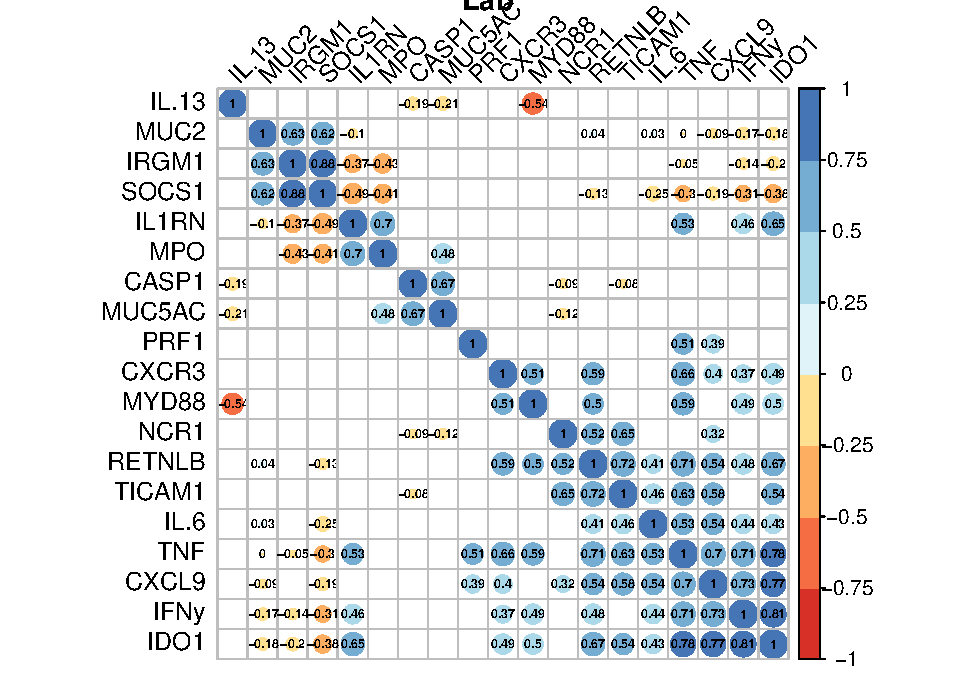
\includegraphics{Testing_normalization_imputation_order_files/figure-latex/unnamed-chunk-6-1.pdf}

\begin{Shaded}
\begin{Highlighting}[]
  \CommentTok{\#Add significance level to the correlogram}
\CommentTok{\#remove the values that are insignificant}
\end{Highlighting}
\end{Shaded}

\hypertarget{correlation-of-non-normalized-and-imputed-gene-expression-data-results}{%
\subsubsection{2. Correlation of non-normalized and imputed gene
expression data,
Results:}\label{correlation-of-non-normalized-and-imputed-gene-expression-data-results}}

\begin{enumerate}
\def\labelenumi{\alph{enumi}.}
\tightlist
\item
  positive correlations between MUC2, IRGM1, SOCS1
\item
  positive correlations between IL1RN, MPO
\item
  positve correlations between CASP1, MUC5AC
\item
  positve correlations between CXCR3, MYD88
\item
  positive correlations between RETNLB, TICAM1, IL.6, TNF, CXCL9, IFNy,
  IDO1
\item
  positive correlations between IL1RN and TNF, IFN\textless{} and IDO1
\item
  negative correlations between IRGM1, SOCS2 and IL1RN, MPO
\item
  negative correlations between group MUC2, IRGM1, SOC1 vs IL.6, TNF,
  CXCL9, IFNy and IDO1
\item
  negative correlations between IL.13 and CASP1, MUC5AC and MYD88
\end{enumerate}

\hypertarget{correlation-of-normalized-data-no-imputation}{%
\subsection{3. Correlation of normalized data (no
imputation)}\label{correlation-of-normalized-data-no-imputation}}

\begin{Shaded}
\begin{Highlighting}[]
\CommentTok{\#ΔCt (sample) = Ct(reference gene) {-} Ct(gene of interest) }

\NormalTok{calculate\_delta\_ct }\OtherTok{\textless{}{-}} \ControlFlowTok{function}\NormalTok{(df, HKG) \{}
  \CommentTok{\# Extract the column of the housekeeping gene}
\NormalTok{  reference\_gene }\OtherTok{\textless{}{-}}\NormalTok{ df[[HKG]]}
\NormalTok{  Mouse\_ID }\OtherTok{\textless{}{-}}\NormalTok{ df}\SpecialCharTok{$}\NormalTok{Mouse\_ID}
\NormalTok{  g }\OtherTok{\textless{}{-}}\NormalTok{ df[, }\FunctionTok{colnames}\NormalTok{(df) }\SpecialCharTok{\%in\%}\NormalTok{ Genes\_v]}

\NormalTok{  delta\_ct }\OtherTok{\textless{}{-}} \FunctionTok{sapply}\NormalTok{(g, }\ControlFlowTok{function}\NormalTok{(gene) reference\_gene }\SpecialCharTok{{-}}\NormalTok{ gene)}
\NormalTok{  delta\_ct }\OtherTok{\textless{}{-}} \FunctionTok{as.data.frame}\NormalTok{(}\FunctionTok{cbind}\NormalTok{(Mouse\_ID, delta\_ct))}
  \FunctionTok{return}\NormalTok{(delta\_ct)}
\NormalTok{\}}

\CommentTok{\# more positive = higher expression }

\CommentTok{\# Use the function}
\NormalTok{norm\_field }\OtherTok{\textless{}{-}} \FunctionTok{calculate\_delta\_ct}\NormalTok{(field, }\StringTok{"GAPDH"}\NormalTok{)}

\NormalTok{norm\_lab }\OtherTok{\textless{}{-}} \FunctionTok{calculate\_delta\_ct}\NormalTok{(lab, }\StringTok{"PPIB"}\NormalTok{)}

\NormalTok{norm\_g }\OtherTok{\textless{}{-}} \FunctionTok{rbind}\NormalTok{(norm\_field, norm\_lab)}

\NormalTok{hm\_norm }\OtherTok{\textless{}{-}}\NormalTok{ hm }\SpecialCharTok{\%\textgreater{}\%}
\NormalTok{    dplyr}\SpecialCharTok{::}\FunctionTok{select}\NormalTok{(}\SpecialCharTok{{-}}\FunctionTok{all\_of}\NormalTok{(Genes\_v)) }\SpecialCharTok{\%\textgreater{}\%}
    \FunctionTok{left\_join}\NormalTok{(norm\_g, }\AttributeTok{by =} \StringTok{"Mouse\_ID"}\NormalTok{)}

\FunctionTok{rm}\NormalTok{(result, norm\_g)}
\end{Highlighting}
\end{Shaded}

\hypertarget{correlations-normalised-genes-no-imputation}{%
\subsubsection{Correlations normalised genes (no
imputation)}\label{correlations-normalised-genes-no-imputation}}

\begin{Shaded}
\begin{Highlighting}[]
\NormalTok{lab }\OtherTok{\textless{}{-}}\NormalTok{ hm\_norm}\SpecialCharTok{\%\textgreater{}\%}
    \FunctionTok{filter}\NormalTok{(origin}\SpecialCharTok{==} \StringTok{"Lab"}\NormalTok{)}

\NormalTok{gene\_correlation }\OtherTok{\textless{}{-}} \FunctionTok{sapply}\NormalTok{(lab[,Genes\_v], as.numeric)}

\CommentTok{\# draw correlation between the genes}
\NormalTok{gene\_correlation }\OtherTok{\textless{}{-}} \FunctionTok{as.matrix}\NormalTok{(}\FunctionTok{cor}\NormalTok{(gene\_correlation, }
                                  \AttributeTok{use=}\StringTok{"pairwise.complete.obs"}\NormalTok{))}

\CommentTok{\# matrix of the p{-}value of the correlatio}
\NormalTok{p.mat }\OtherTok{\textless{}{-}} \FunctionTok{cor.mtest}\NormalTok{(gene\_correlation)}

\FunctionTok{corrplot}\NormalTok{(gene\_correlation, }
         \AttributeTok{method =} \StringTok{"circle"}\NormalTok{,  }\CommentTok{\#method of the plot, "color" would show colour gradient}
         \AttributeTok{tl.col =} \StringTok{"black"}\NormalTok{, }\AttributeTok{tl.srt=}\DecValTok{45}\NormalTok{, }\CommentTok{\#colour of labels and rotation}
         \AttributeTok{col =} \FunctionTok{brewer.pal}\NormalTok{(}\AttributeTok{n =} \DecValTok{8}\NormalTok{, }\AttributeTok{name =}\StringTok{"RdYlBu"}\NormalTok{), }\CommentTok{\#colour of matrix}
         \AttributeTok{order=}\StringTok{"hclust"}\NormalTok{, }\CommentTok{\#hclust reordering}
         \AttributeTok{p.mat =}\NormalTok{ p.mat, }\AttributeTok{sig.level =} \FloatTok{0.01}\NormalTok{, }\AttributeTok{insig =} \StringTok{"blank"}\NormalTok{,}
         \AttributeTok{addCoef.col =} \StringTok{\textquotesingle{}black\textquotesingle{}}\NormalTok{,}
         \AttributeTok{number.cex=}\FloatTok{0.5}\NormalTok{,}
         \AttributeTok{title =} \StringTok{"Lab"}\NormalTok{) }
\end{Highlighting}
\end{Shaded}

\includegraphics{Testing_normalization_imputation_order_files/figure-latex/unnamed-chunk-8-1.pdf}

\begin{Shaded}
\begin{Highlighting}[]
  \CommentTok{\#Add significance level to the correlogram}
\CommentTok{\#remove the values that are insignificant}
\end{Highlighting}
\end{Shaded}

\hypertarget{correlation-of-normalized-not-imputed-gene-expression-data-results}{%
\subsubsection{3. Correlation of normalized (not imputed) gene
expression data,
Results:}\label{correlation-of-normalized-not-imputed-gene-expression-data-results}}

\begin{enumerate}
\def\labelenumi{\alph{enumi}.}
\item
  \begin{itemize}
  \tightlist
  \item
    correlation between IL.13 and TICAM1
  \end{itemize}
\item
  \begin{itemize}
  \tightlist
  \item
    correlation between CXCL9 and TNF, IFNy and IDO1
  \end{itemize}
\item
  \begin{itemize}
  \tightlist
  \item
    correlation between IL1RN, MPO, TNF, IFNy, IDO1
  \end{itemize}
\item
  \begin{itemize}
  \tightlist
  \item
    correlation between NCR1, PRF1, MUC2, IRGM1, SOCS1, CXCR3, CASP1
  \end{itemize}
\item
  \begin{itemize}
  \tightlist
  \item
    correlation between MUC5AC and CXCL9, IL1RN, MUC2, CXCR3, IL.16
  \end{itemize}
\item
  \begin{itemize}
  \tightlist
  \item
    correlation between MYD88 and IL.13, TICAM1
  \end{itemize}
\end{enumerate}

\hypertarget{correlation-of-1st-normalized-and-sequentially-imputed-gene-expression-data}{%
\subsection{4. Correlation of 1st normalized and sequentially imputed
gene expression
data}\label{correlation-of-1st-normalized-and-sequentially-imputed-gene-expression-data}}

\begin{Shaded}
\begin{Highlighting}[]
\NormalTok{hm\_genes }\OtherTok{\textless{}{-}}\NormalTok{ hm\_norm[,}\FunctionTok{c}\NormalTok{(}\StringTok{"Mouse\_ID"}\NormalTok{, Genes\_v)]}


\NormalTok{genes }\OtherTok{\textless{}{-}}\NormalTok{ hm\_genes[, }\SpecialCharTok{{-}}\DecValTok{1}\NormalTok{]}

\CommentTok{\#init \textless{}{-} mice(genes, maxit = 0)}
\end{Highlighting}
\end{Shaded}

Error in edit.setup(data, setup, \ldots) : \texttt{mice} detected
constant and/or collinear variables. No predictors were left after their
removal.

The treshold for colinearity in the package ``MICE'' is set to a max
correlation of 0.99 by default.

The normalised gene expression values present a maximum correlation of

\begin{Shaded}
\begin{Highlighting}[]
\FunctionTok{max}\NormalTok{(gene\_correlation[gene\_correlation }\SpecialCharTok{\textless{}} \DecValTok{1}\NormalTok{], }\AttributeTok{na.rm =} \ConstantTok{TRUE}\NormalTok{)}
\end{Highlighting}
\end{Shaded}

\begin{verbatim}
## [1] 0.9843948
\end{verbatim}

between genes.

I can't run mice as genes become ``too'' correlated.

I can't get this to work:
\url{https://github.com/amices/mice/issues/278}

\hypertarget{corrrelation-of-1st-imputed-and-sequentially-normalized-gene-expression-data}{%
\subsection{5. Corrrelation of 1st imputed and sequentially normalized
gene expression
data}\label{corrrelation-of-1st-imputed-and-sequentially-normalized-gene-expression-data}}

\begin{Shaded}
\begin{Highlighting}[]
\NormalTok{field }\OtherTok{\textless{}{-}}\NormalTok{ hm\_imp }\SpecialCharTok{\%\textgreater{}\%}
\NormalTok{    dplyr}\SpecialCharTok{::}\FunctionTok{filter}\NormalTok{(origin }\SpecialCharTok{==} \StringTok{"Field"}\NormalTok{)}

\NormalTok{lab }\OtherTok{\textless{}{-}}\NormalTok{ hm\_imp }\SpecialCharTok{\%\textgreater{}\%}
\NormalTok{    dplyr}\SpecialCharTok{::}\FunctionTok{filter}\NormalTok{(origin }\SpecialCharTok{==} \StringTok{"Lab"}\NormalTok{)}

\CommentTok{\#ΔCt (sample) = Ct(reference gene) {-} Ct(gene of interest) }

\CommentTok{\# more positive = higher expression }

\CommentTok{\# Use the function}
\NormalTok{norm\_field }\OtherTok{\textless{}{-}} \FunctionTok{calculate\_delta\_ct}\NormalTok{(field, }\StringTok{"GAPDH"}\NormalTok{)}

\NormalTok{norm\_lab }\OtherTok{\textless{}{-}} \FunctionTok{calculate\_delta\_ct}\NormalTok{(lab, }\StringTok{"PPIB"}\NormalTok{)}

\NormalTok{norm\_g }\OtherTok{\textless{}{-}} \FunctionTok{rbind}\NormalTok{(norm\_field, norm\_lab)}

\NormalTok{hm\_norm }\OtherTok{\textless{}{-}}\NormalTok{ hm }\SpecialCharTok{\%\textgreater{}\%}
\NormalTok{    dplyr}\SpecialCharTok{::}\FunctionTok{select}\NormalTok{(}\SpecialCharTok{{-}}\FunctionTok{all\_of}\NormalTok{(Genes\_v)) }\SpecialCharTok{\%\textgreater{}\%}
    \FunctionTok{left\_join}\NormalTok{(norm\_g, }\AttributeTok{by =} \StringTok{"Mouse\_ID"}\NormalTok{)}
\end{Highlighting}
\end{Shaded}

\hypertarget{correlations-normalised-genes-no-imputation-1}{%
\subsubsection{Correlations normalised genes (no
imputation)}\label{correlations-normalised-genes-no-imputation-1}}

\begin{Shaded}
\begin{Highlighting}[]
\NormalTok{lab }\OtherTok{\textless{}{-}}\NormalTok{ hm\_norm}\SpecialCharTok{\%\textgreater{}\%}
    \FunctionTok{filter}\NormalTok{(origin}\SpecialCharTok{==} \StringTok{"Lab"}\NormalTok{)}

\NormalTok{gene\_correlation }\OtherTok{\textless{}{-}} \FunctionTok{sapply}\NormalTok{(lab[,Genes\_v], as.numeric)}

\CommentTok{\# draw correlation between the genes}
\NormalTok{gene\_correlation }\OtherTok{\textless{}{-}} \FunctionTok{as.matrix}\NormalTok{(}\FunctionTok{cor}\NormalTok{(gene\_correlation, }
                                  \AttributeTok{use=}\StringTok{"pairwise.complete.obs"}\NormalTok{))}

\CommentTok{\# matrix of the p{-}value of the correlatio}
\NormalTok{p.mat }\OtherTok{\textless{}{-}} \FunctionTok{cor.mtest}\NormalTok{(gene\_correlation)}

\FunctionTok{corrplot}\NormalTok{(gene\_correlation, }
         \AttributeTok{method =} \StringTok{"circle"}\NormalTok{,  }\CommentTok{\#method of the plot, "color" would show colour gradient}
         \AttributeTok{tl.col =} \StringTok{"black"}\NormalTok{, }\AttributeTok{tl.srt=}\DecValTok{45}\NormalTok{, }\CommentTok{\#colour of labels and rotation}
         \AttributeTok{col =} \FunctionTok{brewer.pal}\NormalTok{(}\AttributeTok{n =} \DecValTok{8}\NormalTok{, }\AttributeTok{name =}\StringTok{"RdYlBu"}\NormalTok{), }\CommentTok{\#colour of matrix}
         \AttributeTok{order=}\StringTok{"hclust"}\NormalTok{, }\CommentTok{\#hclust reordering}
         \AttributeTok{p.mat =}\NormalTok{ p.mat, }\AttributeTok{sig.level =} \FloatTok{0.01}\NormalTok{, }\AttributeTok{insig =} \StringTok{"blank"}\NormalTok{,}
         \AttributeTok{addCoef.col =} \StringTok{\textquotesingle{}black\textquotesingle{}}\NormalTok{,}
         \AttributeTok{number.cex=}\FloatTok{0.5}\NormalTok{,}
         \AttributeTok{title =} \StringTok{"Lab"}\NormalTok{) }
\end{Highlighting}
\end{Shaded}

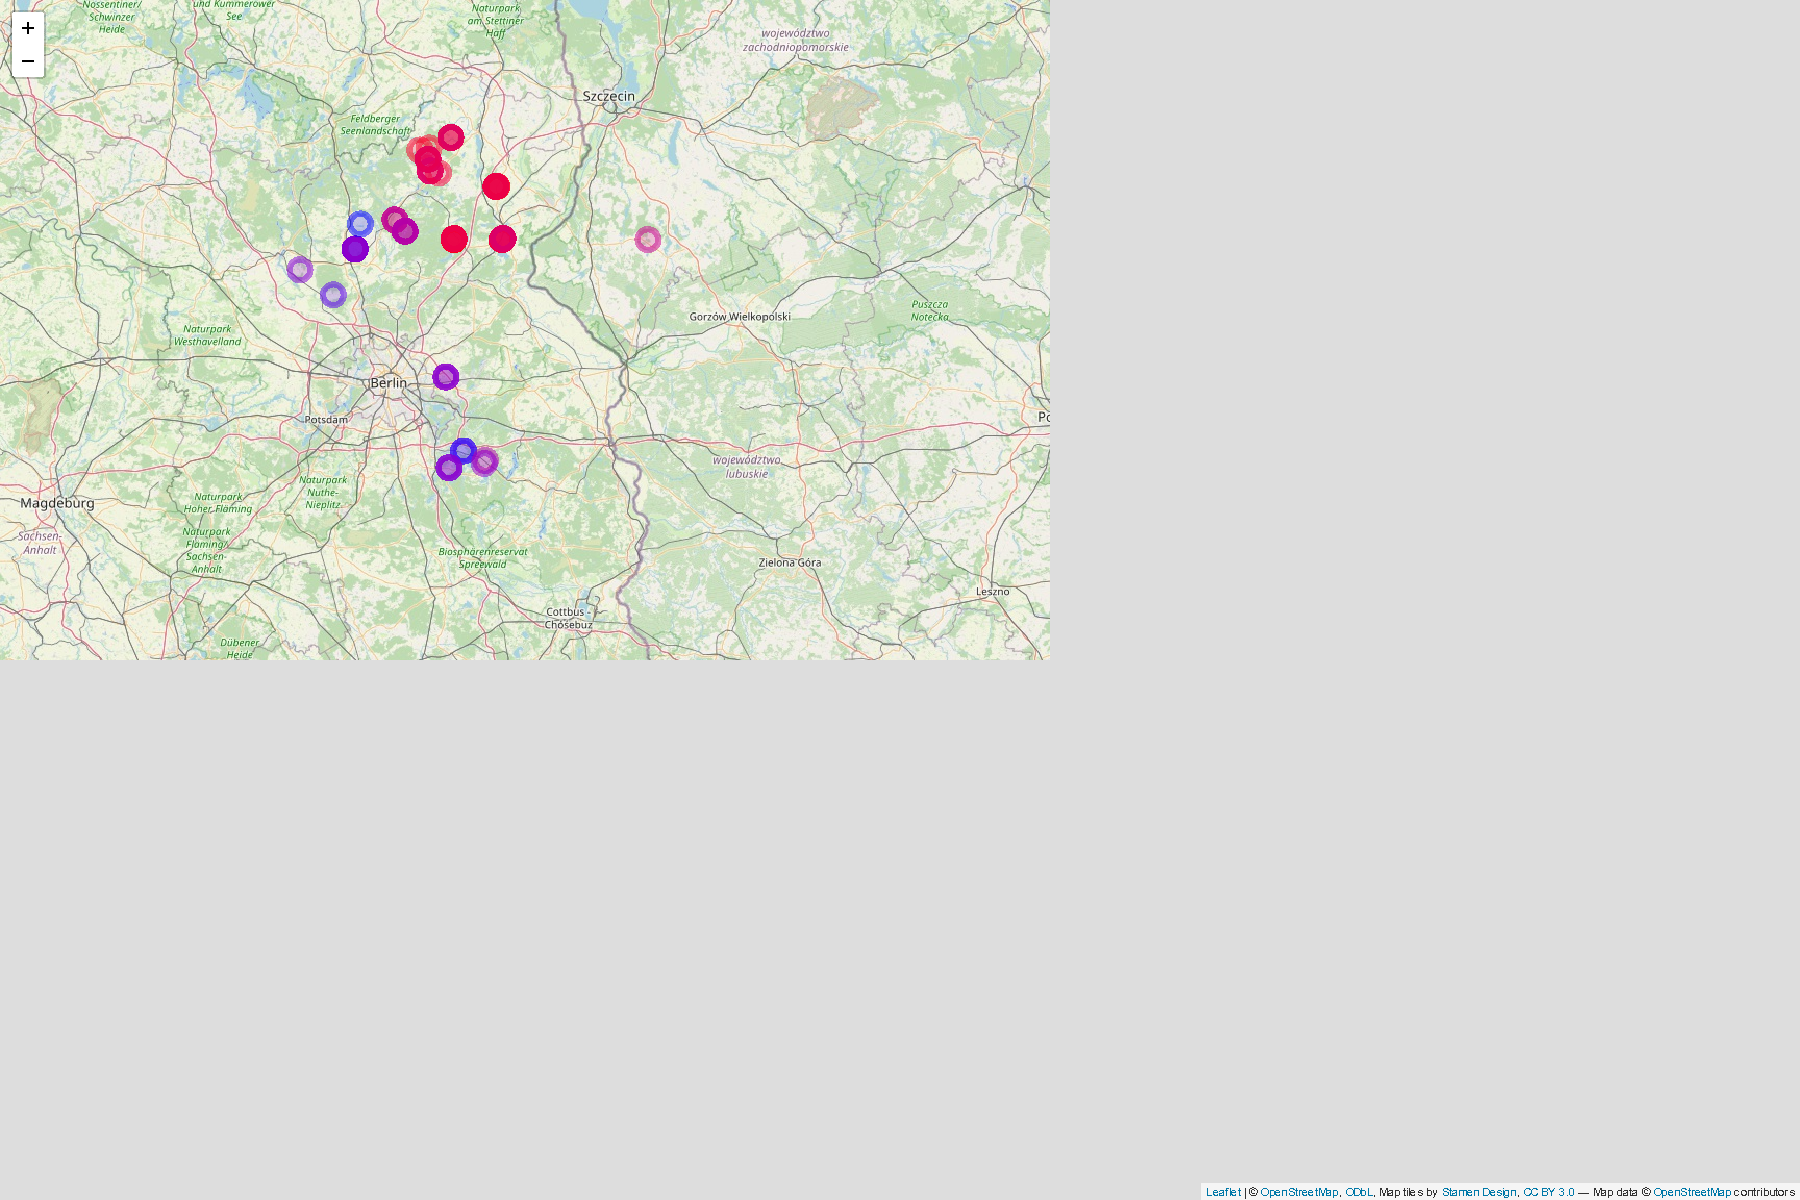
\includegraphics{Testing_normalization_imputation_order_files/figure-latex/unnamed-chunk-12-1.pdf}

\begin{Shaded}
\begin{Highlighting}[]
  \CommentTok{\#Add significance level to the correlogram}
\CommentTok{\#remove the values that are insignificant}
\end{Highlighting}
\end{Shaded}


\end{document}
